\documentclass[english]{article}
\usepackage[T1]{fontenc}
\usepackage[latin9]{inputenc}
\usepackage{graphicx}
\usepackage{babel}
%\usepackage{multicol}
\begin{document}

\parskip=3mm
\parindent=0mm


\begin{center}
\textbf{{\huge Mass Modelling of Globular Clusters in the Milky Way}}
\end{center}

\textbf{{\LARGE 1. Introduction}}

(Formula el problema, se describe lo mas importante que se ha hecho, se menciona que se va a hacer)

\textbf{{\LARGE 2. Theoretical Framework}}


- Cumulos globulares (definiciones, propiedades, formacion, y evolucion, poblaciones estelares, etc)

\textbf{{\Large 2.1 Globular Clusters}}

Typical galaxies all around the Universe hold different structures such as stellar systems of between $ 10^{2} $ and $ 10^{6} $ stars which orbit their galactic core. We call these interesting systems star clusters and they are basically divided into two main types: Open Clusters and \textbf{Globular Clusters}.

Globular clusters are very massive stellar systems that can contain from thousands to millions of stars in a nearly spherical distribution. These stellar systems are composed of old stars and they do not contain gas or dust. 

\textbf{{\Large 2.2 Stellar Systems Dynamics}}

(we focus on globular clusters)

\textbf{{\Large 2.3 Scenario and Observatios}}

\textbf{{\Large 2.4 Simulations}}

\textbf{{\LARGE 3. Observations and Analysis}}

- Describir todo el experimento de observacion

- Describir los datos

- Reduccion

- Extraccion

- Calibracion

- Espectros y photo

- RVSAO y determinacion de velocidades radiales

\textbf{{\Large 3.1 Observational Procedures}}

Under supervision of proffesor Juan Carlos Mu\~noz Cuartas and with three other undergraduate students from the University of Antioquia a trip to the OPD (Pico dos Dias Observatory) was made to Brazil in May 2014, besides the observational experience for the students, the main purpose of the trip was to get important data for the proyect "Dynamics and mass models of the central region of globular clusters in the local Milky Way"

The spectroscopic data allows us to determine the velocity dispersion profile in the inner region of globular clusters; while the photometric data allows us to study the surface brightness distribution for them. We can use all of this information to infer the properties of the globular clusters' mass distribution and build complete dynamical models and therefore infer the amount of dark matter present in the globular clusters (if there is any).

\textbf{{\large 3.1.1 Spectroscopic data}}

The first two days (May 14th and 15th) we took the spectroscopic data in the telescope P\&E with a diameter of 1.6m. The main instrument was the Cassegrain spectrograph with a CCD Ikon-L camera and Filters BVR. The software we used was the recently installed software TCSPD which is built in a LabView environment for Windows (2010)

We made the observations of dome flats, certain globular clusters of the milky Way organized by the best observation times using Simbad and Stellarium for the estimations of the coordinates and times respectivley. We also took calibration stars data, flat fields, different calibration lamps, bias frames and the necessary images to calibrate the instrument.

Here some of the objects we observed organized by "chunks":

\begin{center}
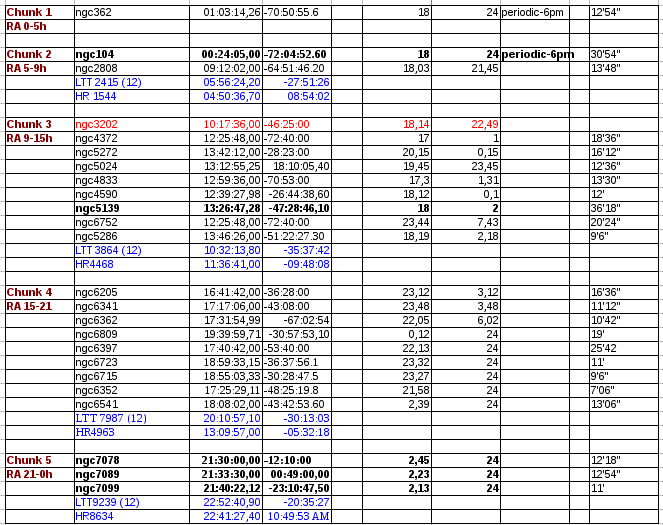
\includegraphics[scale=0.5]{9.png}

\textit{\textbf{Figure 1:}} Chunks
\end{center}

Now, our set up configuration for the spectrograph was the following:

Diffraction grating of 900 lines per mm, a CCD IkonL and the central wavelength for the observations of 8500 Angstroms (for the first day) with rotation of the slit 90°, +45° and -45°.

On May 14th, we used the slit of 2.52" and obtained data for the globular clusters: NGC-5020, NGC-5272, NGC-4833, NGC-4590, NGC-5139, NGC-5286, NGC-6752, NGC-6397, NGC-6723, NGC-6715 and NGC-6541 using exposition times of 600 and 900 seconds. We also observed the calibration stars: HR-4963 and HR-4468 with 7 and 5 seconds. As it was the first day, we needed to be very careful in calibrating our instruments on order to have the objects in the right focus, we also made the rotation of the slit to use all the diffraction angles of the observations and our comparison lamps were of Ne-Ar.

On May 15th, we used the slit of 3.0" and observed the following objects: NGC-2802, NGC-5024, NGC-4590, NGC-5139, NGC-5286, NGC-5272, NGC-6362, NGC-6397, NGC-6723, NGC-6502, NGC-6541, NGC-7078, NGC-7099, the stars HR-4468 and HR-7950 and we also observed Mars for pedagogical reasons. We used pretty much the same exposition times than the day before, this time though, our comparison lamps were or He-Ar. All the data we took was in FITS format (Flexible Image Transfer System).

\textbf{{\large 3.1.2 Photometric Data:}}

The photometric data were acquired in four days, from May 16th to May 19th. 

On May 16th, we took all the calibration images, consisting of 20 bias frames with an exposition time of 0,00001 seconds; also 22, 11, 11, 20 and 10 flat frames for the B,I,R.U.V filters respectively, their exposition times differed . 

May 17th was a terrible night for observations because the sky was too cloudy and the only useful data we could get were flat field images for the filters I,R and V that we could use to fix 


\begin{center}
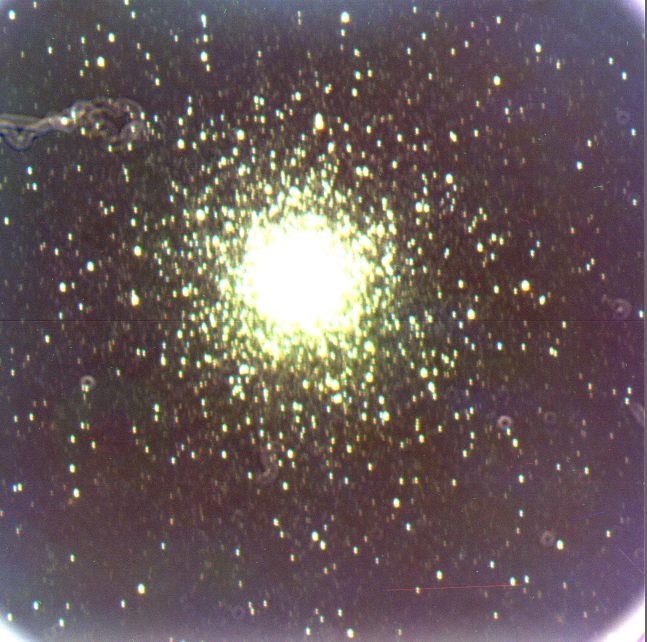
\includegraphics[scale=0.5]{ngc_5139_dirty.png}

\textit{\textbf{Figure:}} Dirty NGC5139 to visualize noice and the need for a proper reduction
\end{center}
------------------------

\textbf{{\Large 3.2 First steps for Analysis}}

Our first goal in starting the analysis of all the relevant data was to organize all the images in order to reduce the time required to make the reductions. For every day the calibrations images, trash, calibration stars and objects were separated and they were given their correct names as they were in the headers and compared with the information sheets we filled at the time we were doing the observations. With the use of an account on the galaxy.udea.edu.co cluster, for proper and quicker analysis and safety of the data, all the files were correctly organized.

The next step was the reduction of all the images with the calibration files for each day, I started the photometric data to acquire certain skills in the use of IRAF because the reduction of the spectroscopic data was to be a little more complex and needed a deeper understanding of IRAF packages. 

I started with the cluster NGC-5139 because we got lots of data for that cluster in OPD and also because Omega Centauri is a well known globular cluster since it is the largest in our galaxy and we can get a lot of information from the web. The photometry was made by the two methods, PSF photometry and Aperture Photometry, even though the magnitudes are quite different, the calibration constant between the two methods gave me a good relation between them and made me trust the photometry results.

After the photometry of that cluster, the most relevant part of the reduction was to be made. The reduction of the spectroscopic data (May 14th and 15th), the methods for these reductions are quite special and are the most relevant part of the analysis because that is our most valuable information. The reduction was to be made very carefully because a good spectroscopic analysis depends upon a good reduction of the data. 

As with the photometric data, the first procedures were made for the Cluster NGC5139 to understand and master the techniques of the reduction and extractions.


\textbf{{\Large 3.3 Photometry}}

\textbf{{\Large 3.4 Spectroscopy}}

\textbf{{\large 3.4.1 Spectroscopic Reduction}}

- First we make a Superbias combining all the bias frames and then we subtract it from all the lamp, targets and flat field frames.

- It was important to analize the flats to see which ones are saturated, we consider that values over 65,000 counts (using implot) show saturated data. The ones that we could trust for May 14th were ten images called flats\_0012 to flats\_0021.

- The pre-superflat is made using the median given the number of images.

- We need to make a trimming in all images because there are some regions in the images that show unexpected luminosity, this is probably due to border errors in the camera or the obturator time of relaxation. The zones we decided to cut were:

[0-100] and [575 to the end]

- A critical step is the creation of a response function, this is made by collapsing the pre-superflat to one column using blkavg. The useful image for the creation of the Superflat is done by combining this column with blkrep. This gives us an image that's uniformly distributed in the dispersion axis with the following IRAF commands.

blkavg MasterFlat.fits[1:475,*] AvgFlatCols 475 1

blkrep AvgFlatCols AvgFlatColsMaster 475 1

- The pre-superflat is now divided by the response function we created (AvgFlatColsMaster) and this gives us the Superflat that we will use to reduce our data.

- Finally, the task we use to remove the cosmic rays is lacos, and it gives very accurate results, as it shows the "mask" image with the removed cosmic rays.

\textbf{{\large 3.4.2 Extraction}}

Once the reduction is ready, we can proceed with the extraction of the spectra of the calibration stars and also the spectra of the stars in the clusters, this procedure is made with the task apall.

Taking special care of correctly choosing the background, and with the following parameter configuration:

b\_number: 100

background: fit

weight: vairance

saturate: 65215

rdnoise: 6

gain: 1

Interactively, one must choose very precisely the background regions to extract the spectrum and do the fitting routines with different orders until the best results are reached.

The extraction of the spectrum for the calibration lamps is done with apsum, which is very similar to apall.

\textbf{{\large 3.4.3 Wavelength calibrations}}

The wavelength calibration is made many tasks of IRAF like Identify, Refspec and Dispcor. First, with identify I use the interactive window in IRAF to select some prominent lines in the spectrum and assign them their correct wavelength using the theoretic spectrum of the lamp. In this case our calibration lamps were Ne-Ar (for May 14th) and He-Ar (for May 15th)  and OPD observatory provided us the theoretic distribution of emission lines of them.

Using "m" to select the larger lines and typing the wavelength, the task creates a file stored in a new folder "database" with the pixels with their corresponding values in units of Angstroms. After that, the targets were to be calibrated with these files so it is necessary to edit their header to assign them the reference frames. It is enough to change the REFSPEC1 image header on each lamp file in order to do the wavelength calibration. 

The task that actually does the calibration on wavelength is dispcor, it is only necessary to run the task over all the targets with their own calibrated arc to get the calibrated spectrum which is the useful and important file to make the analysis of the width of the lines and their redshift.

\textbf{{\large 3.4.4 Flux Calibration}}

The aim is to calibrate the CCD chip response, spectrograph+telescope throughput and allow for atmospheric extinction. The result is a spectrum as observed from outside the atmosphere with an ideal uniformly sensitive detector+telescope+spectrograph. Basically, what the flux calibration does is, it takes from a tabular compilation the energy distribution of the standard star, it corrects this energy distribution for wavelength-dependent atmospheric extinction, it compares it to the energy distribution of the observed spectrum and derives from such a comparison the function that gives the response of our system for every wavelength.

The flux calibration takes place in three parts: Calibrating from the standard star, calculating the sensitivity function of the instrument, and finally, applying the calibration to the spectra. We will use the task observatory to determine observatory parameters, standard to flux calibrate each standard star, and sensfunc to finally determine the wavelength response and the solution will be applied to the spectra by the task calibrate.

In the first part, the calibration is made with one of the stars that are already included in IRAF, there are many stars so there's quite a good amount of options to choose. So the first task is the task standard. The observatory parameter is specified as LNA which is in IRAF's database. 

\textbf{The task standard}

The task standard determines calibration pass-bands and writes them to a file called std. The thrick here is to specify the location of the the input extinction and flux calibration files. To do that, I edit the parameters of standard with the following routes:

Extinction file:                              onedstds\$/ctioextindt.dat

Directory containing calibration data:   onedstds\$ctionewcal/

Starname in calibration list:                l9239

Where I chose the Star l9239 because it has the spectral range that we use in our calibration Stars. And running the task interactively would be enough for this step.

\textbf{The task sensfunc}

Standard task just recorded response of each standard star so the next step is to put the results together and find a proper wavelength dependence of instrumental sensitivity and atmosphere transparency using the task sensfunc. It creates an image with a default name sens.0001. IRAF needs to have some general idea of atmospheric extinction before to start, so I set again extinct onedstds\$ /ctioextinct.dat.

Now, running the task interactively and taking into account that the function used to fit the instrumental response will be usually of very high order. A good idea is to use spline3 fitting (:function spline3) with some 20 pieces, i.e. (:order 20).
Finally q exists the sensfunc task and writes the sens.0001 image.

\textbf{The task calibrate}

The solution to each star to be calibrated is done with the task calibrate. Editting the parameters of calibrate to set the appropriate extinction table: extinct onedstds\$ /ctioextinct.dat would be enough for this purpose. The task is run over all the wavelength calibrated spectra which had their airmass and other parameters appropriately set by the eso.set procedure. And finally it gives the flux-calibrated spectra ready for the relevant analysis concerning radial velocities.

After the flux calibration, I notice that the extremes of the spectra have irregularities but that can be cut because they don't have any relevant information.

For the star calibration I cut from 0 to 45 and from 1860 to the end, using imcopy:

\begin{center}
imcopy flux\_calib\_star\_fits[45:1860,*] cut\_flux\_calib\_star.fits
\end{center}

In order to normalize the spectrum, first I find the maximum value in the spectrum using minmax and then I divide the whole image by this value.

Now, to create the Ascii table from the spectrum I need to first convert my image to a 1D image using the task scopy and setting format=onedspec

Now, with the image ready in 1D, I use the task wspectext to create the Ascii table like this:

\begin{center}
wspectext ready\_flux\_star.0001.fits normal\_cut\_flux\_star\_calib.txt
\end{center}

\textbf{{\Large 3.5 RVSAO and radial velocity determination}}



\textbf{{\LARGE 4. Modelling}}



\textbf{{\LARGE 5. Conclusions}}






\end{document}